\chapter{RESULTS}

\graphicspath{ {./results/} }
%%%%%%%% This line gets rid of page number on first page of text
\thispagestyle{empty}

%%%%%%%%%%%%%

The result section details essential findings from our research study and prototype testing, including multiple iterations and user testing to analyze different variations.

\section{Visual Analysis}

The critical finding from the research highlights that the representations learned by the VGG16 image recognition model are highly amenable to visualization, in large part because they are representations of visual concepts. 

Although a wide variety of techniques are under development in the research and visual analytics community, we covered three of the most accessible and useful ones:

\begin{enumerate}
\item Visualizing heatmaps of class activation
\item Visualizing filter patterns
%\item Visualizing intermediate activations
\end{enumerate}

For all three methods, we use the VGG16 model, a convolutional neural network based model trained on the imagenet database that we introduced in the previous section.

\section*{Image Receptivity of Feature Map}

This step helps to understand precisely which part of an image identified to belong to a specific class or category (class names known to VGG16), and thus allows localizing objects in images.

We feed the following image of a group of bee-eater sitting on a tree branch as an input image.

%Input image ~\ref{fig:myFig}.
\begin{figure}[htbp]
\centering
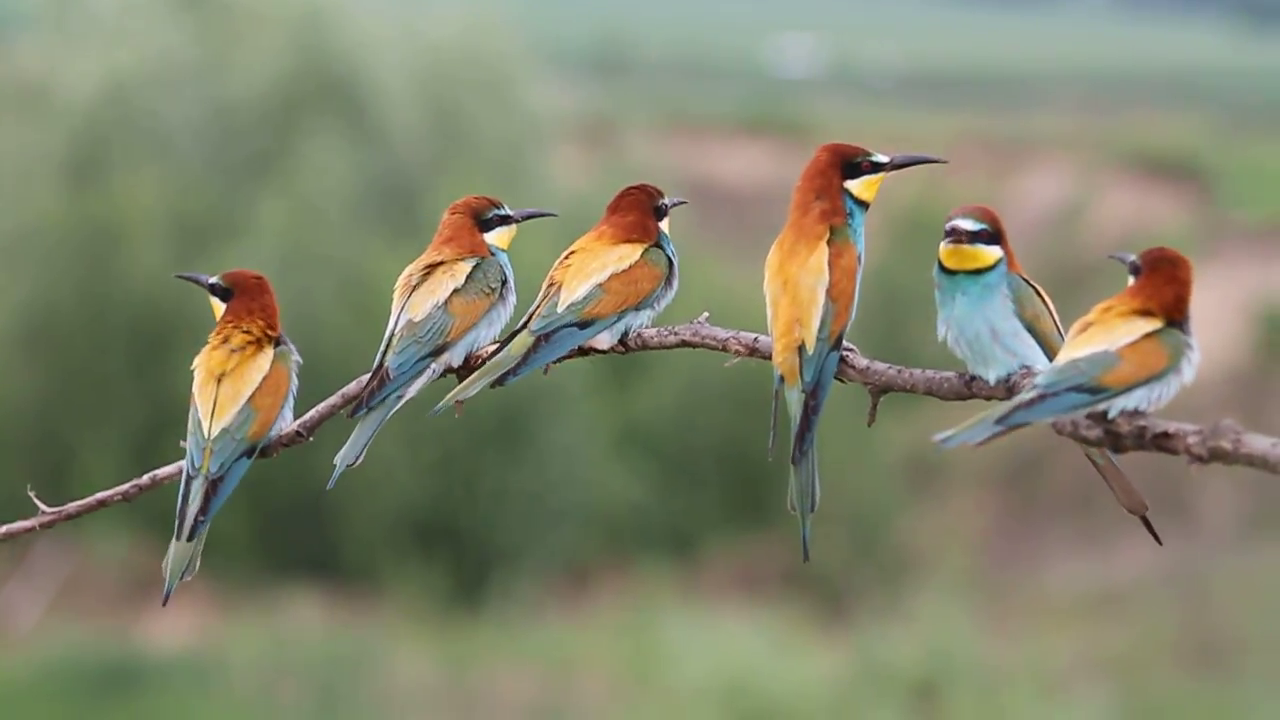
\includegraphics[width=0.80\textwidth]{images/colorful-group-of-birds-get-together_vkmuak6_e__F0000.png}
\caption{An image of colorful group of birds uploaded by the user}
\label{fig:myFig}
\end{figure}

>>> [IMAGE] Rooster Image Self Prototype (XAI: UNDERSTANDING, VISUALIZING AND INTERPRETING DEEP LEARNING MODELS)

%Class activation heatmap~\ref{fig:heatmap-1}.
\begin{figure}[htbp]
\centering
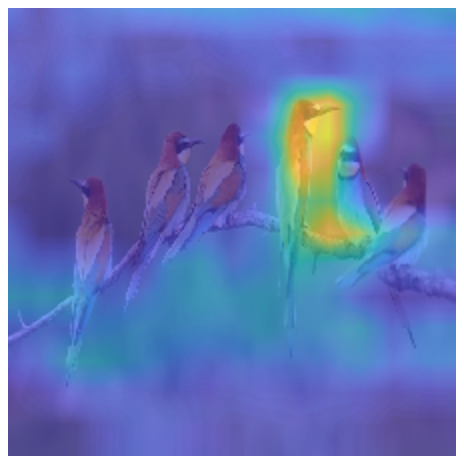
\includegraphics[width=0.50\textwidth]{images/heatmap-class-activations.png}
\caption{Image Receptivity}
\label{fig:heatmap-1}
\end{figure}

\section*{Activation Graph}

This step helped to understand when fed with an input image, how successful layers of the network transformed the input image. It also helped get an idea of the meaning of the individual network filters.

\iffalse
\section*{Visualizing filters}

This step that visualizes set of patterns, which is useful to understand precisely what visual patterns or concepts each filter in a layer is receptive to.
\fi

Our visualization technique helped to answer two important questions:

\begin{itemize}
\item  Why did the network think this image contained a bee-eater?
\item Where is the bee-eater located in the picture?
\end{itemize}

In particular, what is most exciting to note is that the head region of the fourth bird, which is the largest of all six birds are strongly activated: this is probably how the network can tell the difference between bee-eater and any other bird.

\section{User Study}

\iffalse
RESULTS
WE USE localization approaches like CAM APPROACH ONLY + ....

Visualizing intermediate activations¶

Visualizing intermediate activations consists in displaying the feature maps that are output by various convolution and pooling layers in a network, given a certain input (the output of a layer is often called its "activation", the output of the activation function). This gives a view into how an input is decomposed unto the different filters learned by the network. These feature maps we want to visualize have 3 dimensions: width, height, and depth (channels). Each channel encodes relatively independent features, so the proper way to visualize these feature maps is by independently plotting the contents of every channel, as a 2D image. Let's start by loading the model that we saved in section 5.2:

Visualizing convnet filters
inspect the filters learned by convnets is to display the visual pattern that each filter is meant to respond to. This can be done with gradient ascent in input space: applying gradient descent to the value of the input image of a convnet so as to maximize the response of a specific filter, starting from a blank input image. The resulting input image would be one that the chosen filter is maximally responsive to.

Visualizing heatmaps of class activation¶
We will introduce one more visualization technique, one that is useful for understanding which parts of a given image led a convnet to its final classification decision. This is helpful for "debugging" the decision process of a convnet, in particular in case of a classification mistake. It also allows you to locate specific objects in an image.
This general category of techniques is called "Class Activation Map" (CAM) visualization, and consists in producing heatmaps of "class activation" over input images. A "class activation" heatmap is a 2D grid of scores associated with an specific output class, computed for every location in any input image, indicating how important each location is with respect to the class considered. For instance, given a image fed into one of our "cat vs. dog" convnet, Class Activation Map visualization allows us to generate a heatmap for the class "cat", indicating how cat-like different parts of the image are, and likewise for the class "dog", indicating how dog-like differents parts of the image are.
\fi

\iffalse
\section{Visualization Outcome}
\section{Statistical Analysis}
\section{Visual Analysis}


\section{User Testing}
\section{Performance Testing}
\fi
